\chapter{Algoritmy řešící [n,k]-Mastermind}

\section{Kategorie algoritmů}
% přidat definici algoritmu, který řeší mastermind - vytvoří posloupnost kódů, která končí tajným kódem s nejlepším ohodnocením. 
Algoritmy řešící hru Mastermind lze rozdělit do dvou kategorií, \textbf{deterministické} a \textbf{nedeterministické}. Deterministický algoritmus pro dva shodné stavy volí další krok vždy jednoznačně. Nemůže se tedy stát, že by deterministický algoritmus pro dva stejné vstupy vrátil odlišné výsledky. Nedeterministické algoritmy naproti tomu mohou mít v každém stavu na výběr z více následujících kroků. Volit mohou například podle nějakého pravděpodobnostního rozdělení. Není tedy zaručeno, že pro stejný vstup vrátí vždy identický výsledek.

Hlavní předností deterministických algoritmů je záruka výsledku. Na druhou stranu ale tyto typy algoritmů mohou mít velikou časovou složitost, protože jsou často založeny na procházení všech možností pokračování. To se snaží řešit nedeterministické algoritmy, které hledají rovnováhu mezi časovou složitostí a dobrými výsledky. 

V této práci budeme zkoumat pouze deterministické algoritmy. 

% šlo by zmínit výhody a nevýhody (ne)deterministických algoritmů
% Popsat algoritmy, které hrají pouze kandidáty????


\section{Deterministické algoritmy}
% mozna napsat pozdeji ... Všechny deterministické algoritmy, které budeme srovnávat ...

\subsubsection{stav hry}

%Tajný kód je tedy kandidát v každém kole hry. 
Stav hry budeme znázorňovat množinou kódů $K \subset H_{n,k}$. Prvky této množiny jsou kódy, které by mohly být tajným kódem podle informací dostupných z tahů a ohodnocení. Nejprve popíšeme vztah mezi stavy, který bude určitým způsobem odpovídat změně stavu v průběhu hry. 

%který nám bude sloužit k definování hran. Vazbu a přechod mezi stavy hry budeme zakreslovat do grafu. Nejprve popíšeme vztah mezi vrcholy (stavy), který nám bude sloužit k definování hran.
% může platit, že $(K,K_{u,r_1}) = (K,K_{v,r_2})$ pro nějaké u,v,r_1,r_2
% potomek může být i on sám. Chce to ale dobře definovat, abychom se necyklili. 
\begin{definice}[Potomek]\label{potomek}
  % Uvažujme [n,k]-Mastermind s nějakým tajným kódem $v\in H_{n,k}$. 
  Nechť $S$ je množina všech ohodnocení v $H_{n,k}$. Nechť $K$ je podmnožina $H_{n,k}$, $ u \in H_{n,k}$ je kód a $r \in S$ ohodnocení. Potomka $K$, vzhledem ke kódu $u$ a ohodnocení $r$ definujeme jako množinu 
  \[K_{u,r} = \{w \in K \mid s(u,w) = r\}.\] 
\end{definice}

\begin{pozn}
    Potomkem $K$, vzhledem ke kódu $u$ nazýváme množinu $K_{u,r}$ pro nějaké $r \in S$. Potomkem $K$ nazýváme množinu $K_{u,r}$ pro nějaké $u\in H_{n,k}$ a $r \in S$. 
\end{pozn}

\begin{pozn}
    Všimněme si, že $K_{u,r} \subset K \hspace{3px}\forall u\in H_{n,k} \hspace{3px}\forall r\in S$. Navíc pro každou množinu $K \subset H_{n,k}$ a kód $u \in H_{n,k}$ platí
    \[K = \bigcup_{r\in S} K_{u,r}\]
    protože pro každý kód $w \in K$ platí, že $w \in K_{u, s(u,w)}$ z definice potomka.
    %, tedy že $w$ náleží do potomka $K$ vzhledem ke kódu $u$ a ohodnocení $s(u,w)$. 
\end{pozn}
% Definujeme orientovaný graf hry s podmnožinami $H_{n,k}$ jako vrcholy. 

Průběh hry budeme reprezentovat grafem s podmnožinami $H_{n,k}$ jako vrcholy a orientovanými hranami mezi vrcholy a jejich potomky. Výchozí stav hry je vždy celá množina $H_{n,k}$, protože každý kód může být tajným kódem. 

\begin{definice}[Graf \text{[n,k]-Mastermindu}]
  Uvažujeme množinu vrcholů $\mathcal{V} = \mathcal{P}(H_{n,k})$ a množinu orientovaných hran $\mathcal{E}$ mezi vrcholy a jejich potomky. Cestu definujeme jako posloupnost navazujících hran. Definujeme $V \subset \mathcal{V}$ jako množinu vrcholů, do kterých vede cesta z vrcholu $H_{n,k}$. Graf [n,k]-Mastermindu definujeme jako indukovaný podgraf grafu $(\mathcal{V}, \mathcal{E})$ množinou $V$. Hranu $(K, K_{u,r})$ budeme značit jako hranu $(u,r)$ z vrcholu $K$.
\end{definice}
 
\begin{pozn}
    Mezi dvěma vrcholy může vést více hran, jak je vidět na obrázku \ref{fig22prvnitah}, který zobrazuje potomky $H_{2,2}$ vzhledem ke všem kódům a ohodnocením. Pro přehlednost jsou potomci vzhledem ke stejnému kódu zakresleny u sebe, protože odpovídají možným dalším stavům v případě zvolení tohoto kódu jako dalšího pokusu. 
    
    %Vrchol také může být potomkem sebe samého. 
\end{pozn}


\begin{figure}[h!]
    \centering
    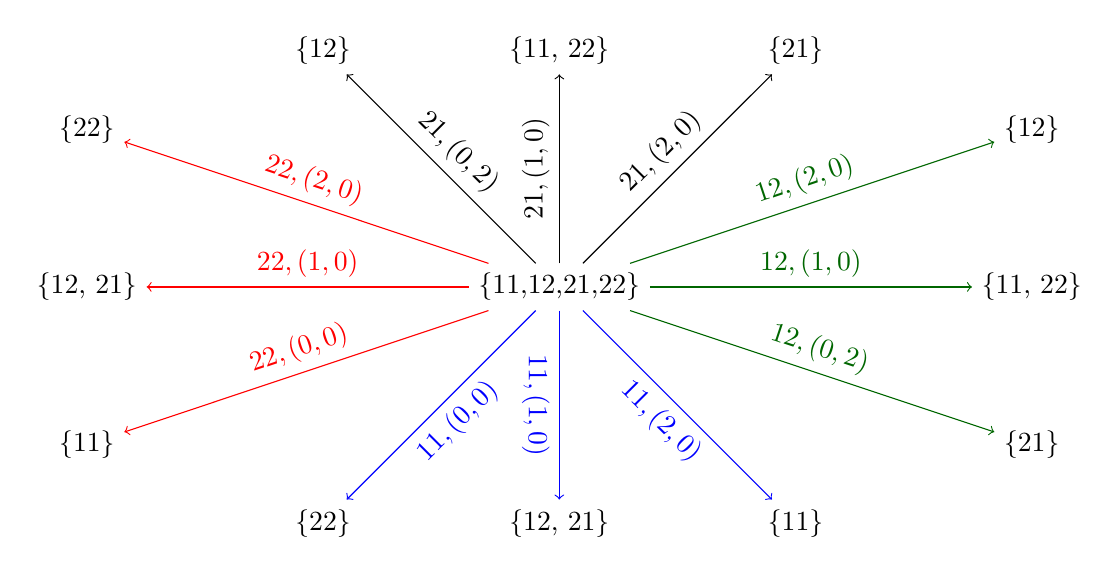
\begin{tikzpicture}
    \node (1) at (0,0) {\{11,12,21,22\}};
    
    \node (2) at (-3,-3) {\{22\}};
    \draw[->,blue] (1) -- (2) node[pos=0.5, below, sloped] {$11,(0,0)$};
    \node (3) at (0,-3) {\{12, 21\}};
    \draw[->,blue] (1) -- (3) node[pos=0.5, below, sloped] {$11,(1,0)$};
    \node (4) at (3,-3) {\{11\}};
    \draw[->,blue] (1) -- (4) node[pos=0.5, below, sloped] {$11,(2,0)$};
    
    \node (5) at (6,-2) {\{21\}};
    \draw[->,black!60!green] (1) -- (5) node[pos=0.5, above, sloped] {$12,(0,2)$};
    \node (6) at (6,0) {\{11, 22\}};
    \draw[->,black!60!green] (1) -- (6) node[pos=0.5, above, sloped] {$12,(1,0)$};
    \node (7) at (6,2) {\{12\}};
    \draw[->,black!60!green] (1) -- (7) node[pos=0.5, above, sloped] {$12,(2,0)$};

    \node (8) at (-3,3) {\{12\}};
    \draw[->] (1) -- (8) node[pos=0.5, above, sloped] {$21,(0,2)$};
    \node (9) at (0,3) {\{11, 22\}};
    \draw[->] (1) -- (9) node[pos=0.5, above, sloped] {$21,(1,0)$};
    \node (10) at (3,3) {\{21\}};
    \draw[->] (1) -- (10) node[pos=0.5, above, sloped] {$21,(2,0)$};

    \node (11) at (-6,-2) {\{11\}};
    \draw[->,red] (1) -- (11) node[pos=0.5, above, sloped] {$22,(0,0)$};
    \node (12) at (-6,0) {\{12, 21\}};
    \draw[->,red] (1) -- (12) node[pos=0.5, above, sloped] {$22,(1,0)$};
    \node (13) at (-6,2) {\{22\}};
    \draw[->,red] (1) -- (13) node[pos=0.5, above, sloped] {$22,(2,0)$};


    \end{tikzpicture}
    \caption{Graf všech potomků $H_{2,2}$}
    \label{fig22prvnitah}
\end{figure}

\begin{definice}[Strom průběhu \text{[n,k]-Mastermindu}]
  Strom průběhu hry definujeme jako podgraf grafu [n,k]-Mastermindu s následujícími vlastnostmi. 
  \begin{enumerate}
      \item Z každého vrcholu vedou hrany pouze do potomků vzhledem k jednomu danému kódu. 
  \end{enumerate}
\end{definice}

\begin{definice}[Stav]\label{stav}
   Nechť $u_i, i\in \{1,2,\dots m\}$ jsou kódy a $r_i = (b_i,w_i)$ jsou ohodnocení. Stav definujeme jako posloupnost $((u_1, r_1), \dots, (u_m, r_m))$. Počáteční stav definujeme jako prázdnou posloupnost.
\end{definice}

\begin{definice}[kandidát]\label{kandidat}
  Nechť $\left((u_1, r_1), (u_2,r_2), \dots, (u_j,r_j)\right), u_i \in H_{n,k}, r_i \in \N _0 \times \N _0$ je stav. Řekneme, že kód $u \in H_{n,k}$ je kandidát, pokud $s(u,u_i) = r_i \hspace{5px} \forall i \in \{1, \dots j\}$. Pro počáteční stav je kandidátem každý kód $u \in H_{n,k}$. Řekneme, že stav je prázdný, pokud je množina kandidátů tohoto stavu prázdná. 
  % Tohle není přesné - Pro prázdný stav řekneme, že každý kód $u \in H_{n,k}$ je kandidát. Množinu všech kandidátů budeme značit $K$.
\end{definice}

\begin{definice}[Strom \text{[n,k]-Mastermindu}]
  Orientovaný strom průběhu hry definujeme na množině stavů. Kořen je počáteční stav. Hrany označíme $(u, r)$ pro kód $u$ a nějaké ohodnocení $r$. Ze stavu $A = \left((u_1, r_1), (u_2,r_2), \dots, (u_j,r_j)\right)$ do stavu $B = \left((w_1, s_1), (w_2,s_2), \dots, (w_l,s_l)\right)$ vede hrana právě tehdy, když $l = j+1$ a $\forall i \in \{1,2,\dots, j\} \colon (u_i, r_i) = (w_i, s_i)$. Tuto hranu značíme $(w_l, s_l)$. Prázdné stavy a hrany do prázdných stavů ve stromu neuvažujeme.
\end{definice}

\begin{definice}[Podstrom strategie \text{[n,k]-Mastermindu}]
  Konečný stav jsou ty neprázdné stavy, které mají poslední člen stavu roven $(u,(n,0))$ pro nějaký kód $u$.
  Podstrom strategie definujeme takový souvislý podgraf stromu [n,k]-Mastermindu, jehož všechny listy jsou konečné stavy. 
\end{definice}
\begin{pozn}
    Konečné stavy jsou právě takové stavy, které mají pouze jednoho kandidáta a odpovídají nalezení tajného kódu v průběhu hry mastermind. 
\end{pozn}
\begin{pozn}
    Stavy budeme také označovat množinou kandidátů pro tento stav. Množina kandidátů neurčuje jednoznačně stav (například prohozením prvků stavu bychom došli do stejné množiny kandidátů). Naopak stav jednoznačně určuje množinu kandidátů. 
\end{pozn}

% možná to není potřeba
%\begin{lemma}[Jednoznačnost hrany]
 %   Nechť $(V, E)$ je graf a $K \in V$ je vrchol. Potom z $K$ vede právě jedna hrana 
%\end{lemma}

Prvky aktuálního stavu hry $K\subset H_{n,k}$ nazýváme kandidáty. 
\begin{definice}[Kandidát]
    Uvažujme [n,k]-Mastermind s nějakým tajným kódem $v\in H_{n,k}$. Nechť 
    \[P = \left((u_1, s_v(u_1)), (u_2,s_v(u_2)), \dots, (u_j,s_v(u_j))\right), u_i \in H_{n,k}, \]
    % r_i \in \N _0 \times \N _0
    jsou tahy s ohodnocením vzhledem ke kódu $v$. Řekneme, že $u \in H_{n,k}$ je kandidát, pokud $u \in K$, kde $K$ je konec cesty $P$ z vrcholu $H_{n,k}$. $K$ nazýváme množinu všech kandidátů tohoto stavu. 
\end{definice}
\begin{pozn}
    Nechť $P = \left((u_1, s_v(u_1)), (u_2,s_v(u_2)), \dots, (u_j,s_v(u_j))\right), u_i \in H_{n,k}$ jsou tahy s ohodnocením, $K$ je konec cesty a $u \in K$ je kandidát. Potom $\forall i \in \{1,2,\dots j\}$ platí $s(u,u_i) = s_v(u_i)$. Tajný kód $v$ je tedy kandidát pro každý stav hry. 
\end{pozn}




% tato definice možná ani není potřeba, protože s ní dále nepracuji
%\begin{definice}[Rozdělení]
 %   Pro $K \subset H_{n,k}$ definujeme rozdělení vzhledem ke kódu $u$ jako množinu potomků $K$, vzhledem ke kódu $u$. $R_{K,u} = \{K_{u,r} \mid r \in S\}$. 
%\end{definice}


\subsubsection{Obecný algoritmus}
Nyní přistoupíme k popisu skupiny deterministických algoritmů řešící hru [n,k]-Mastermind. Využijeme k tomu dvě funkce, valuaci a strategii.
% U této definice si nejsem jistý, jak to smyslupně definovat. Vazba "která lz e vyjádřit pomocí potomků" se mi moc nelíbí - definovat valuaci a až potom jednokrokové valuace
\begin{definice}[Valuace]
    Nechť $G = (V,E)$ je graf [n,k]-Mastermindu a $K \in V$ je vrchol. Potom valuaci vzhledem k množině $K$ definujeme jako funkci $f_K(u) \colon H_{n,k} \to \mathbb{R}$.
\end{definice}
Valuace bude v algoritmech sloužit pro vyčíslení vhodnosti kódu $u$ jako dalšího pokusu pro stav $K\subset H_{n,k}$. Tato hodnota bude obvykle záviset na potomcích $K$ vzhledem ke kódu $u$. Potomci $K$ vzhledem ke kódu $u$ totiž určují možné následující stavy v případě, kdy zvolíme kód $u$ jako další pokus. Valuace nám umožňuje ohodnotit kód podle toho, jak dobré jsou jeho následující stavy. 

\begin{prikl}\label{prjednokrokfce}
    Funkce $f_K$ je příklad valuace, která kódu $u$ přiřadí očekávaný počet kódů potomka $K$ vzhledem ke kódu $u$.
    % jednokrokov8 funkce je taková, která kódu $u$ přiřadí hodnotu, která lze vyjádřit pomocí potomků $K$ vzhledem ke kódu $u$.
    \begin{align*}
        f_K \colon H_{n,k} &\to \mathbb{R} \\
        u &\mapsto \sum_{r\in S}\frac{|K_{u,r}|}{|K|}|K_{u,r}| 
    \end{align*}
    Pro $K = H_{2,2}$ z obrázku \ref{fig22prvnitah} má $f_{K}$ konstantní hodnotu $\frac{3}{2}$.
\end{prikl}
% množinu kandidátů na tajný kód
Obecně valuace nemusí být omezená na následující vrstvu. Mohla by odkazovat na očekávaný počet kódů vrcholu o dvě či více vrstev dál. 

\begin{definice}[Strategie]
    Nechť $\mathcal{F} = \{f_K\colon H_{n,k} \to \mathbb{R} \mid K \subset H_{n,k}\}$ je prostor valuací. Potom strategii definujeme jako zobrazení $F \colon \mathcal{F} \to \mathbb{R}$. 
\end{definice}
% Strategie určitým způsobem slouží k výběru následujícího kódu. 
%Zjednodušeně řečeno slouží k určení, 
Strategie v této práci bude určovat, zda chceme vybírat kódy s vyšší nebo nižší hodnotou valuace.
%Použití bude popsáno níže v popisu algoritmu \ref{alg-default}. 

\begin{prikl}\label{prstrategie}
    Funkce $F$ je strategie, která funkci $f_K \in \mathcal{F} = \{f_K\}$ přiřadí její maximální hodnotu na $H_{n,k}$.
    \[F(f_K) =  \max_{u\in H_{n,k}}\{f_K(u)\}\]
    Strategie je dobře definovaná, protože maximum na konečné množině reálných čísel má vždy jednoznačnou hodnotu.
\end{prikl}

Deterministické algoritmy popisujeme jako algoritmy, které pro následující pokus vybírají kód podle zvolené valuace a strategie. Postup je znázorněn v algoritmu \ref{alg-default}.

% \subsection{Varianty algoritmů}





%Nechť \[P = \left((u_1, r_1), (u_2,r_2), \dots, (u_j,r_j)\right), u_i \in H_{n,k}, r_i \in \N _0 \times \N _0\] jsou tahy s ohodnocením a $K$ je konec cesty $P$ z vrcholu $H_{n,k}$. 

%Potom jednokrokové strategie volí další kód ten, který minimalizuje respektive maximalizuje funkci $f_K$. Pokud je těchto kódů více, zvolí kód, který je zároveň kandidát cesty $P$. Pokud výběr stále není jednoznačný, algoritmus zvolí lexikograficky nejnižší kód. 

\begin{algorithm}[h!]
\begin{algorithmic}[1]  % [1] způsobí, že číslujeme kroky algoritmu
\Function{Solve$[n, k, \mathcal{F}, F]$}{$v$}
    \State $K \gets H_{n,k}$ 
    \State $j \gets 0$
    \State $r_0 \gets (0,0)$
    \While {$r_j \neq (n,0)$} \hfill \mbox{(dokud hra není dohrána)}
        \State $j \gets j + 1$ 
	\State $U \gets \{u \in H_{n,k} \mid f_K(u) = F(f_K)\}$
        \If{$U \cap K \neq \emptyset$}
            \State $u_j \gets$ lexikograficky nejmenší $u \in U \cap K$
	\Else
		\State $u_j \gets$ lexikograficky nejmenší $u \in U$
	\EndIf
        \State $r_j \gets s(u_j, v)$ \hfill \mbox{(ohodnocení pokusu)}
        \State $K \gets K_{u_j,r_j}$
    \EndWhile
    \State \Return $u_j, j$ \hfill \mbox{($u_j$ je tajný kód, $j$ je počet pokusů)}
\EndFunction
\end{algorithmic}
\caption{Algoritmus řešící [n,k]-Mastermind}
\label{alg-default}
\end{algorithm}

Písmenem $K$ značíme množinu kandidátů na tajný kód pro aktuální stav hry (cestu pokusů s ohodnocením). Začínáme s $K = H_{n,k}$. Aktuální číslo pokusu značí $j$, $u_j$ je kód, který algoritmus zvolí jako $j$-tý pokus a $r_j$ je ohodnocení $u_j$ vzhledem k tajnému kódu $v$. Množina $U$ značí kódy, ve kterých valuace $f_K$ nabývá určitou optimální hodnotu danou strategií $F$. Z této množiny algoritmus vybírá další pokus $u_j$. Ve chvíli, kdy existuje kandidát v množině $U$ ($U\cap K \neq \emptyset$), algoritmus zvolí ten, který je lexikograficky nejmenší. Jinak algoritmus volí lexikograficky nejmenší kód z $U$. 

Aby byla strategie $F$ použitelná v algoritmu, musí platit následující podmínka. 
\[\forall K \in V \hspace{5px} \exists u \in H_{n,k} \colon F(f_K) = f_K(u)\]
Pokud by tato podmínka nebyla splněna, mohlo by se stát, že množina $U$ bude prázdná a algoritmus nedokáže zvolit další pokus.

% šlo by napsat pro dvojice funkce f, funkcionál F
%\begin{veta}[Správnost algoritmu \ref{alg-default}]
 %   Algoritmus \ref{alg-default}
%\end{veta}

\begin{tvrz}[Počet ohodnocení]
Nechť $n\in \mathbb{N}, k\in \mathbb{N}, k \geq 3$. Potom počet všech možných ohodnocení kódů v $H_{n,k}$ je $\frac{n^2 + 3n}{2}$.
\end{tvrz}
\begin{dukaz}
Pro $b \leq n,\hspace{3px} b \neq n-1$ černých kolíčků existuje $n-b+1$ možností na počet bílých kolíčků podle tvrzení \ref{tvrzohodnoceni}. Pro $b = n-1$ existuje pouze jedno ohodnocení. Součtem přes počet černých kolíčků dostáváme následující počet možností ohodnocení.
    \[|S| = (n+1) + n + (n-1)  + \dots + 3 + 1 + 1 \]
Vzorcem pro součet aritmetické řady se dobereme k výsledku.
    \[|S| = \frac{(n+1)(n+2)}{2} - 1 \]
    \[|S| = \frac{n^2 + 3n}{2}\]
\end{dukaz}

\begin{tvrz}[Časová složitost algoritmu \ref{alg-default}]
    Uvažujeme případ, kdy $F$ je minimizér/maximizér.
    Algoritmus \ref{alg-default} má časovou složitost
    % \[O( k^n O(f_K))\]
    \[O \left( \sum_{j = 1}^z k^n \cdot m_j \cdot n^2 \cdot \frac{n^2 + 3n}{2}\right)\]
    
\end{tvrz}
\begin{dukaz}
    $k^n$ je počet všech kódů, které musím projít, abych našel ten nejlepší, $m_j$ je maximální počet kandidátů v j-té iteraci, $z$ je maximální počet iterací algoritmu. $\frac{n^2 + 3n}{2}$ je počet všech ohodnocení, $n^2$ je časová složitost ohodnocení.

    Potřebuji ještě limit na počet iterací $z$, horní odhad na $m_j$ a zjistit složitost nalezení průniku $U$ a $K$.
\end{dukaz}

